\section{Introduction}
\label{sec:syn-intro}

The problem of equivalence checking between a functional specification and an
implementation written in a low level imperative language such as C
has been of immense research interest
and has several important applications such as (a) program verification, where
the equivalence checker is used to verify that the C implementation
behaves according to the specification and (b) translation validation, where
the equivalence checker attempts to generate a proof of equivalence across
the transformations (and translations) performed by an optimizing compiler
and more. The verification of a C implementation against its manually written
functional specification through manually-coded refinement proofs has been
performed extensively in the seL4 microkernel \cite{seL4}.
Frameworks for program equivalence proofs have been developed in interactive
theorem provers like Coq \cite{programEquivalenceInCoq} where correlations and invariants
are manually identified during proof codification.
On the other hand, programming languages like Dafny \cite{dafny} offer automated program
reasoning for imperative languages with abstract data types such as sets and arrays.
Such languages perform automatic compile-time checks for manually-specified correctness predicates through
SMT solvers.
% Also, there exists significant prior work on translation validation
% \cite{tvi,tristan_tv_eqsat11,stepp_eqsat_llvm11,eqsat,pec,zuck03,zuck05,heffter05,covac,c_to_verilog,kanade09,lopes16,tvoc_cav05,ddec,semalign,oopsla20,tv_oskernel,namjoshi13}
% across low level programming languages such as C and assembly.
% In most of these applications, soundness in critial,
% i.e., if the equivalence checker determines the programs to be equivalent, then the programs are indeed equivalent
% and evidently has equivalent observable behaviour. On the other hand, a sound equivalence checker may be incomplete
% and fail to prove the programs to be equivalent, even if they were equivalent.

We present \toolName{}, an algorithm to automatically (push-down) search
for a proof of equivalence between a functional specification and its
optimized C implementation. We will demonstrate how \toolName{} is capable of
proving equivalence of multiple equivalent C implementations with vastly
different (a) data layouts (e.g. array, linked list representations of a {\em list})
and (b) algorithmic strategies (e.g. alternate algorithms, optimizations) against
a {\em single} functional specification.
This opens the possibility of regression verification \cite{strichman_regressverify,felsing14},
where \toolName{} can be used to automate verification across software updates that change memory layouts for
data structures and algorithms.
We start by formulating the problem statement and define equivalence in this context.
Next, we shortly introduce bisimulation in the context of program equivalence and list our primary contributions.

\subsection{Problem Setting and Bisimulation}
\label{sec:syn-setting-bisimulation}
We restrict our attention to programs that construct, read, and write
to recursive data structures. In languages like C, pointer and array based
implementations of these data-structures are prone to safety and liveness bugs.
Similar recursive data structures are also available in safer functional langugaes like Haskell,
where algebraic data types (ADTs) \cite{hope} ensure several safety properties.
We define a minimal functional language, called \SpecL{}, that enables the safe
and succint specification of programs manipulating and traversing recursive data structures.

\begin{figure}[H]
\begin{tabular}{cc}
\begin{subfigure}[b]{0.565\textwidth}
\begin{center}
\begin{allLangEnvScript}
~{\tiny \textcolor{mygray}{A0:}}~ type List = LNil | LCons (val:i32, tail:List).
~{\tiny \textcolor{mygray}{A1:}}~
~{\tiny \textcolor{mygray}{A2:}}~ fn mk_list_impl (n:i32) (i:i32) (l:List):List=
~{\tiny \textcolor{mygray}{A3:}}~    if ${\tt i \geq_u n}$ then l
~{\tiny \textcolor{mygray}{A4:}}~    else make_list_impl(n, i+${\tt 1_{i32}}$, LCons(i, l)).
~{\tiny \textcolor{mygray}{A5:}}~
~{\tiny \textcolor{mygray}{A6:}}~ fn mk_list (n:i32):List=
~{\tiny \textcolor{mygray}{A7:}}~    mk_list_impl(n, ${\tt 0_{i32}}$, LNil).
\end{allLangEnvScript}
\end{center}
\caption{\label{fig:llAllocSpec}Spec Program}
\end{subfigure}%
&
\begin{subfigure}[b]{0.435\textwidth}
\begin{center}
\begin{allLangEnvScript}
~{\tiny \textcolor{mygray}{S0:}}~ List mk_list (i32 n) {
~{\tiny \textcolor{mygray}{S1:}}~   List l $\coloneqq$ LNil;
~{\tiny \textcolor{mygray}{S2:}}~   i32  i $\coloneqq$ ${\tt 0_{i32}}$;
~{\tiny \textcolor{mygray}{S3:}}~   while ${\tt \neg (i \geq_{u} n)}$:
~{\tiny \textcolor{mygray}{S4:}}~     l $\coloneqq$ LCons(i, l);
~{\tiny \textcolor{mygray}{S5:}}~     i $\coloneqq$ i + ${\tt 1_{i32}}$;
~{\tiny \textcolor{mygray}{S6:}}~   return l;
~{\tiny \textcolor{mygray}{SE:}}~ }
\end{allLangEnvScript}
\end{center}
\caption{\label{fig:llAllocSpecIR}(Abstracted) Spec IR}
\end{subfigure}%
\\
\begin{subfigure}[b]{0.565\textwidth}
\begin{center}
\begin{allLangEnvScript}
~{\tiny \textcolor{mygray}{B0: }}~ typedef struct lnode {
~{\tiny \textcolor{mygray}{B1: }}~   unsigned val; struct lnode* next; } lnode;
~{\tiny \textcolor{mygray}{B2: }}~ 
~{\tiny \textcolor{mygray}{B3: }}~ lnode* mk_list(unsigned n) {
~{\tiny \textcolor{mygray}{B4: }}~   lnode* l = NULL;
~{\tiny \textcolor{mygray}{B5: }}~   for (unsigned i = 0; i < n; ++i) {                       $\phantom{\mem{} \coloneqq {\tt \mem{}[ \& (\structPointer{\tt p}{\mem{}}{lnode}{val}) \leftarrow i]_{i32}};}$
~{\tiny \textcolor{mygray}{B6: }}~     lnode* p = malloc(sizeof lnode);                       $\phantom{\mem{} \coloneqq {\tt \mem{}[\&  (\structPointer{\tt p}{\mem{}}{lnode}{next}) \leftarrow l]_{i32}};}$
~{\tiny \textcolor{mygray}{B7: }}~     p$\rightarrow$val = i; p$\rightarrow$next = l; l = p;
~{\tiny \textcolor{mygray}{B8: }}~   }
~{\tiny \textcolor{mygray}{B9: }}~   return l;
~{\tiny \textcolor{mygray}{B10:}}~ }
\end{allLangEnvScript}
\end{center}
\caption{\label{fig:llAllocC}C Program with {\tt malloc()}}
\end{subfigure}%
&
\begin{subfigure}[b]{0.435\textwidth}
\begin{center}
\begin{allLangEnvScript}
~{\tiny \textcolor{mygray}{C0:}}~ i32 mk_list (i32 n) {
~{\tiny \textcolor{mygray}{C1:}}~   i32 l $\coloneqq$ ${\tt 0_{i32}}$;
~{\tiny \textcolor{mygray}{C2:}}~   i32 i $\coloneqq$ ${\tt 0_{i32}}$;
~{\tiny \textcolor{mygray}{C3:}}~   while ${\tt i <_{u} n}$:
~{\tiny \textcolor{mygray}{C4:}}~     i32 p $\coloneqq$ malloc$_{\tt C4}$(sizeof lnode);
~{\tiny \textcolor{mygray}{C5:}}~     $\mem{}$ $\coloneqq$ ${\tt \mem{}[ \& (\structPointer{\tt p}{\mem{}}{lnode}{val}) \leftarrow i]_{i32}}$;
~{\tiny \textcolor{mygray}{C6:}}~     $\mem{}$ $\coloneqq$ ${\tt \mem{}[\&  (\structPointer{\tt p}{\mem{}}{lnode}{next}) \leftarrow l]_{i32}}$;
~{\tiny \textcolor{mygray}{C7:}}~     l $\coloneqq$ p;
~{\tiny \textcolor{mygray}{C8:}}~     i $\coloneqq$ i + ${\tt 1_{i32}}$;
~{\tiny \textcolor{mygray}{C9:}}~   return l;
~{\tiny \textcolor{mygray}{CE:}}~ }
\end{allLangEnvScript}
\end{center}
\caption{\label{fig:llAllocCIR}(Abstracted) C IR}
\end{subfigure}%
\\
\end{tabular}
\caption{\label{fig:llAllocSpecAndC}Spec and C programs for constructing a linked list along with their corresponding abstracted intermediate representations.}
\end{figure}

\Cref{fig:llAllocSpec,fig:llAllocC} shows construction of lists in \SpecL{} and C respectively.
The inputs to a \SpecL{} procedure are its well-typed arguments, which may include recursive data structure
values. The inputs to a C procedure are its explicit arguments and the implicit state of program memory
at procedure entry. We lower both \SpecL{} and C programs to a
Three-Address-Code (3AC) style intermediate representation (IR)
as shown in \cref{fig:llAllocSpecIR,fig:llAllocCIR}. For a \SpecL{} program,
(a) all tail-recursive calls are converted to loops in IR while non-tail calls are preserved and
(b) {\tt match} statements are lowered to equivalent \sumDtor{} conditionals.
For a C program, (a) the sizes and memory layouts of both scalar (e.g., {\tt int})
and compound (e.g., {\tt struct}) types are concretized in IR and
(b) all allocation functions (e.g., {\tt malloc}) are annotated with their
allocation site i.e. IR PC (e.g., {\tt malloc$_{\tt C4}$} in \cref{fig:llAllocCIR}).

\subsubsection{Equivalence Definition}
\label{sec:syn-equivalence}
\toolName{} computes equivalence between the IRs of the \SpecL{} and C sources respectively.
Henceforth, we will omit the sources and continue to refer to the IRs as \SpecL{} and C directly.
Given (1) a \SpecL{} program specification $S$, (2) a C implementation $C$,
(3) a precondition $Pre$ that relates the inputs {\tt Input}$_S$ and {\tt Input}$_C$ to $S$ and $C$
respectively, and (4) a postcondition $Post$ that relates the final outputs {\tt Output}$_S$
and {\tt Output}$_C$ of $S$ and $C$ respectively:
$S$ and $C$ are {\em equivalent} if for all possible inputs \sv{Input} and \cv{Input} such that
$Pre(\sv{Input},\cv{Input})$ holds,
$S$'s execution is well-defined on \sv{Input} i.e. \sdef{}, {\em and} C's
memory allocation requests during its execution on \cv{Input} are successful i.e. \cfits{},
then both programs $S$ and $C$ produce outputs
that satisfy $Post$.
$$
Pre(\sv{Input},\cv{Input}) \land \sdef{} \land \cfits{} \Rightarrow Post(\sv{Output},\cv{Output})
$$

\begin{figure}[]
\begin{tabular}{ccc}
\begin{subfigure}[b]{0.27\textwidth}
\begin{center}
{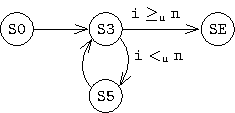
\includegraphics[scale=1]{chapters/figures/figMallocSpecCfg.pdf}}
\vspace{2pt}
\end{center}
\caption{\label{fig:llAllocSpecIRCFG}CFG of \SpecL{} Program}
\end{subfigure}%
&
\begin{subfigure}[b]{0.27\textwidth}
\begin{center}
{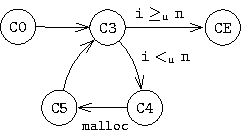
\includegraphics[scale=0.95]{chapters/figures/figMallocCCfg.pdf}}
\vspace{7pt}
\end{center}
\caption{\label{fig:llAllocCCFG}CFG of C Program}
\end{subfigure}%
&
\begin{subfigure}[b]{0.36\textwidth}
\begin{center}
{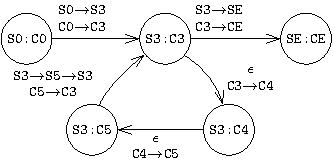
\includegraphics[scale=1]{chapters/figures/figMallocProductCfg.pdf}}
\end{center}
\caption{\label{fig:llAllocProductCFG}CFG of Product Program}
\end{subfigure}%
\\
\end{tabular}
\caption{\label{fig:mallocSpecCFGAndCCFGAndProductCFG}CFG representation for Spec and C IRs shown in \cref{fig:llAllocSpecIR,fig:llAllocCIR}.\\ \Cref{fig:llAllocProductCFG} shows a product-CFG between the CFGs in \cref{fig:llAllocSpecIRCFG,fig:llAllocCCFG}.}
\end{figure}

\begin{table}[H]
\begin{center}
\caption{\label{tab:llproductInv}Node Invariants for Product-CFG in \cref{fig:llAllocProductCFG}}
\setlength{\belowcaptionskip}{-30pt}
\begin{footnotesize}
\begin{tabular}{|c|llll|}
\hline
\tt PC-Pair & \multicolumn{4}{c|} {\tt Invariants} \\
\hline
\hline
${\tt (S0:C0)}$ &
\multicolumn{4}{l|} {\Tstrut ${\tt { \circled{P}}\  n_{S}=n_{C}}$} \\
${\tt (S3:C3)}$ &
\Tstrut  ${\tt {\scriptsize \circled{I1}}\  n_{S}=n_{C}}$ & ${\tt {\scriptsize \circled{I2}}\  i_{S}=i_{C}}$ & ${\tt {\scriptsize \circled{I3}}\  i_{S} \leq_{u} n_{S}}$ & ${\tt {\scriptsize \circled{I4}}\  l_{S}\indEq{}Clist^{lnode}_{m}(l_{C})}$ \\
${\tt (S3:C4)\ (S3:C5)}$ &
\Tstrut  ${\tt {\scriptsize \circled{I5}}\  n_{S}=n_{C}}$ & ${\tt {\scriptsize \circled{I6}}\  i_{S}=i_{C}}$ & ${\tt {\scriptsize \circled{I7}}\  i_{S} <_{u} n_{S}}$ & ${\tt {\scriptsize \circled{I8}}\  l_{S}\indEq{}Clist^{lnode}_{m}(l_{C})}$ \\
${\tt (SE:CE)}$ &
\multicolumn{4}{l|} {\Tstrut  ${\tt {\circled{E}}\  ret_{S}\indEq{}Clist^{lnode}_{m}(ret_{C})}$} \\
\hline
\end{tabular}
\end{footnotesize}
\end{center}
\end{table}

\vspace{-5px}
\Cref{fig:llAllocSpecIRCFG,fig:llAllocCCFG} shows the Control-Flow Graph (CFG) representation
of the \SpecL{} and C programs in \cref{fig:llAllocSpecIR,fig:llAllocCIR} respectively.
Each node represent a PC location of its corresponding program, and each edge represent
transitions between PCs through instruction execution. For brevity, we often represent
a sequence of instructions with a single edge, e.g., in \cref{fig:llAllocCCFG}, the edge
\cpath{5,3} represents the path \cpath{5,6,7,8,3}.
A control-flow edge is associated with an {\em edge condition} (the condition under which that edge is taken),
a {\em transfer function} (how the program state is mutated if that edge is taken),
and a {\em UB assumption} (what condition should be true for the program
execution to be well-defined across this edge).

\subsubsection{Bisimulation Relation}
\label{sec:syn-bisim}
We construct a {\em bisimulation relation} to identify equivalence between two programs.
A bisimulation relation correlates the transitions of $S$ and $C$ in lockstep, such that the
lockstep execution ensures identical observable behavior.
A bisimulation relation between two programs can be represented using a {\em product program}
\cite{covac} and the CFG representation of a product program is called a {\em product-CFG}.
\Cref{fig:llAllocProductCFG} shows a product-CFG, that encodes the lockstep execution
(bisimulation relation) between the CFGs in \cref{fig:llAllocSpecIRCFG,fig:llAllocCCFG}.

\Cref{tab:llproductInv} shows the precondition (labeled \circled{\small P}),
inductive invariants (labeled \circled{\small I}) and postcondition (labeled \circled{\small E})
for the product-CFG in \cref{fig:llAllocProductCFG}. The precondition and postcondition are
provided manually by the user while the intermediate inductive invariants are inferred automatically.
The invariant labeled \circled{\small I4} is an example of a \recursiveRelation{} and represents
the equality between the \SpecL{} \type{List} variable \sv{l} and the \type{List} represented by
chasing \type{lnode} pointers starting at \cv{l}.
Semantically $l_1\indEq{}l_2$ and $l_1=l_2$ are equivalent, `\indEq{}' simply emphasizes the
fact that $l_1$ and $l_2$ are values of (possibly recursive) ADT types.
\lifted{list}{\mem{}}{lnode}{p} is called a {\em lifting constructor} that {\em lifts}
the C pointer value {\tt p} (pointing to an object of type \type{struct lnode}) and the C
memory state \mem{} to a \SpecL{} \type{List} value, and is defined by:
\begin{equation}
\label{eqn:clist}
\begin{split}
U_C:\ &\lifted{list}{\mem{}}{lnode}{p\ctype{i32}} = \sumIf{p=0} \ \sumThen{\cons{LNil}} \\ & \qquad\qquad\ \ \  \sumElse{\cons{LCons}(\structPointer{p}{\mem{}}{lnode}{val}, \lifted{list}{\mem{}}{lnode}{\structPointer{p}{\mem{}}{lnode}{next}})}
\end{split}
\end{equation}
The iterative construction of the product-CFG along with inference of inductive invariants at its nodes are based on
prior work \cite{oopsla20} and discussed briefly in \cref{sec:syn-contribs}. Given a product-CFG
and inferred invariants, the equivalence checker attempts to prove each inductive invariant and
postcondition under the appropiate preconditions for each edge in the product-CFG. These proof
obligations are expressed as relational Hoare triples \cite{relationalHoareLogic,hoareTriple}
and lowered to a first order logic predicate using weakest precondition predicate transformer.
For example, \hoareTriple{\phi_s}{\sv{\rho},\cv{\rho}}{\phi_d}
represents the Hoare triple where $\phi_s$ and $\phi_d$ represents the pre- and postconditions
and (\sv{\rho},\cv{\rho}) represents a product-CFG edge correlating the paths \sv{\rho} and \cv{\rho}
in $S$ and $C$ respectively. The above Hoare triple lowers to the following predicate:
\begin{equation}
\label{eqn:firstOrderFormula}
(\phi_s \land pathcond_{\sv{\rho}} \land pathcond_{\cv{\rho}} \land ubfree_{\sv{\rho}}) \Rightarrow {\tt WP}_{{\sv{\rho},\cv{\rho}}}(\phi_d)
\end{equation}
We will use `\lhs{}' and `\rhs{}' to refer to the antecedant and consequent of the
implication operator `$\Rightarrow$' in \cref{eqn:firstOrderFormula}.
These proof obligations often contains \recursiveRelations{} encoding equality between
arbitrarily-deep recursively data structure values of $S$ and $C$ respectively.
The handling of these proof obligations is a major challenge and forms our primary
contribution as discussed next in \cref{sec:syn-contribs}.
\vspace{-5px}
\subsection{Our Contributions}
\label{sec:syn-contribs}
As previously discussed in \cref{sec:syn-bisim}, showing equivalence through a bisimulation proof
requires three major steps:
\circled{\small 1} An algorithm for construction of a product-CFG by correlating
program executions across the \SpecL{} and C programs respectively,
\circled{\small 2} An algorithm for identification of inductive invariants at correlated PCs and
\circled{\small 3} A proof discharge algorithm for discharging proof obligations containing \recursiveRelations{}.
We base algorithms \circled{\small 1} and \circled{\small 2} on modified versions of counterexample-guided correlation
and invariant inference algorithms\cite{oopsla20}. Our major contributions are as follows:

\begin{itemize}
\setlength{\itemsep}{0px}
\item Proof Discharge Algorithm: Discharging proof obligations (algorithm \circled{\small 3})
involving \recursiveRelations{} is rather challenging and forms our primary contribution.
We describe a {\em sound} proof discharge algorithm capable of tackling proof obligations involving
\recursiveRelations{} using off-the-shelf SMT solvers. Our proof discharge algorithm is also capable of
reconstruction of counterexamples for the original proof query from models returned by the individual SMT queries.
These counterexamples are the backbone of counterexample-guided algorithms for
\circled{\small 1} and \circled{\small 2} steps. As part of our proof discharge procedure,
we reformulate equality of values (i.e. \recursiveRelations{}) as equivalence of their corresponding programs
and discharge these proof queries using a nested (albeit much simpler) bisimulation check.

\item Spec-to-C Equivalence Checker Tool: Our second contribution is \toolName{}, an equivalence checker tool
capable of proving equivalence between a \SpecL{} and a C program automatically. \toolName{} is based on
the Counter tool\cite{oopsla20} and uses an modification of (a) counterexample-guided correlation algorithm for
incremental construction of a product-CFG and (b) counterexample-guided invariant inference algortihm
for inference of inductive invariants at correlated PCs in the (partially constructed) product-CFG.
\toolName{} discharges required verification conditions (i.e. proof obligations) using our Proof Discharge Algorithm.
\end{itemize}

\Cref{sec:syn-examples} walks through our proof discharge algorithm by demonstrating each of its
components using examples. We evaluate our equivalence checking tool \toolName{} in \cref{sec:syn-eval}.
Finally, \cref{sec:syn-limitations} gives an overview of its limitations and \cref{sec:syn-conclusion} concludes our discussion.